\documentclass[11pt]{report}
\usepackage[pdftex]{graphicx}

\usepackage{henrian-basic}
\usepackage{henrian-homework}

\usepackage{amsmath}
\usepackage{float}

\makeHeaders{Machine Learning: Homework 7}

\tolerance=100000

\begin{document}

\begin{itemize}
  \item \textbf{Email}: chrisbrown@utexas.edu
  \item \textbf{EID}: chb595
\end{itemize}

\section{Q-learning}

\subsection{Enviroment}

Figuring out how to quantify the state spaces was the hardest part of the assignment. For the obstacle module, I ended up assigning one label to every combination of adjacent (up/down/left/right) squares that were occupied with obstacles (12, plus 1 for the case where there are no adjacent obstacles).

For the state space of the finish module, there is only one state: the one where you try to get to the end. I thought about having something like a \texttt{floor(log(distance-from-end))} state space; which would allow the learner to worry less about speed if the end of the sidewalk was far off. This actually just made the finish module slower, and didn't make sense in this problem, so I didn't not include this subtlety in the finished product.

I played around with different dimensions of sidewalks and obstacles density, as well as Q-learning algorithm parameters; the results below are each labeled with the parameters.

In each of the plot titles, a means the alpha parameter, g means the discount parameter, and e means the epsilon parameter.
For interpretability of results, I have set the reward for finishing equal to the length of the sidewalk. I played around the amount of the penalty. But for most of the runs below, the penalty was around $-10$.

\begin{figure}[H]
  \centering
  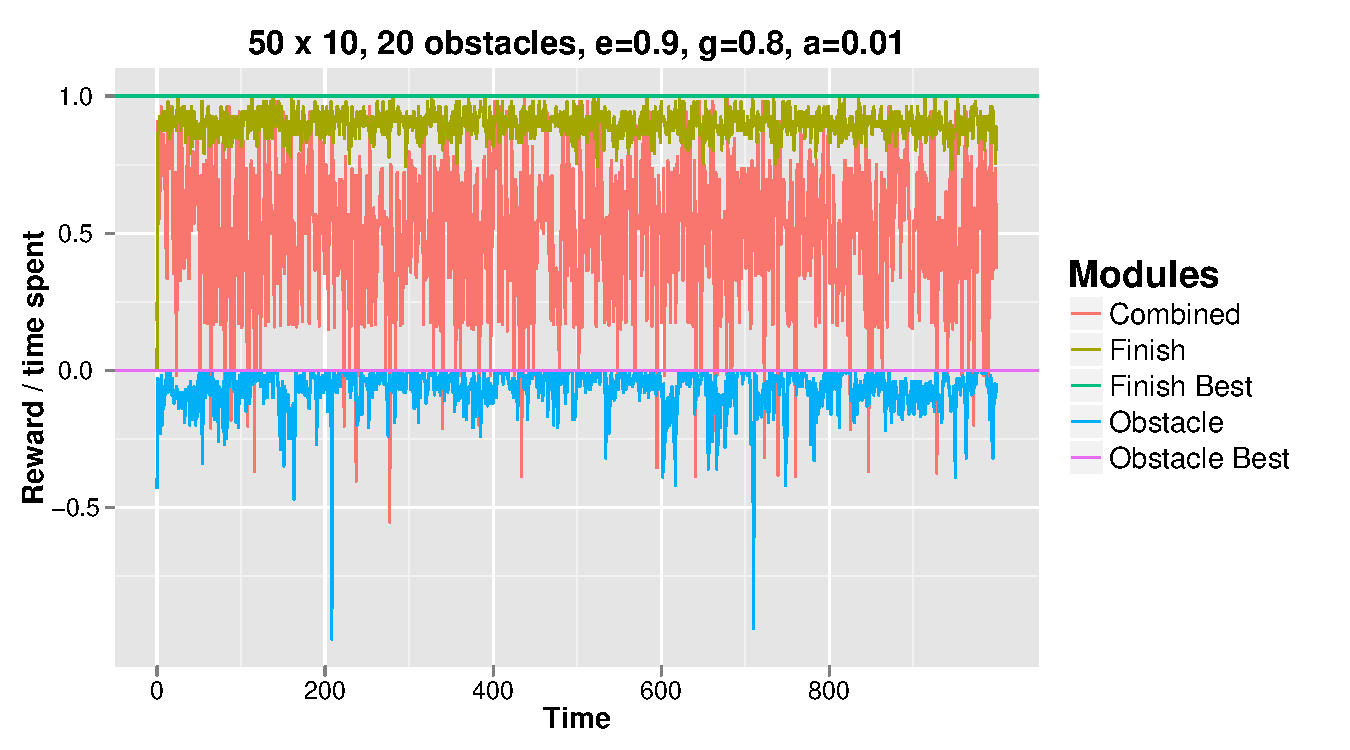
\includegraphics[width=0.95\textwidth]{results/qlearn-s50x10-o20.pdf}
  \caption{epsilon = 0.9}
  \label{fig:ep09}
\end{figure}

\begin{figure}[H]
  \centering
  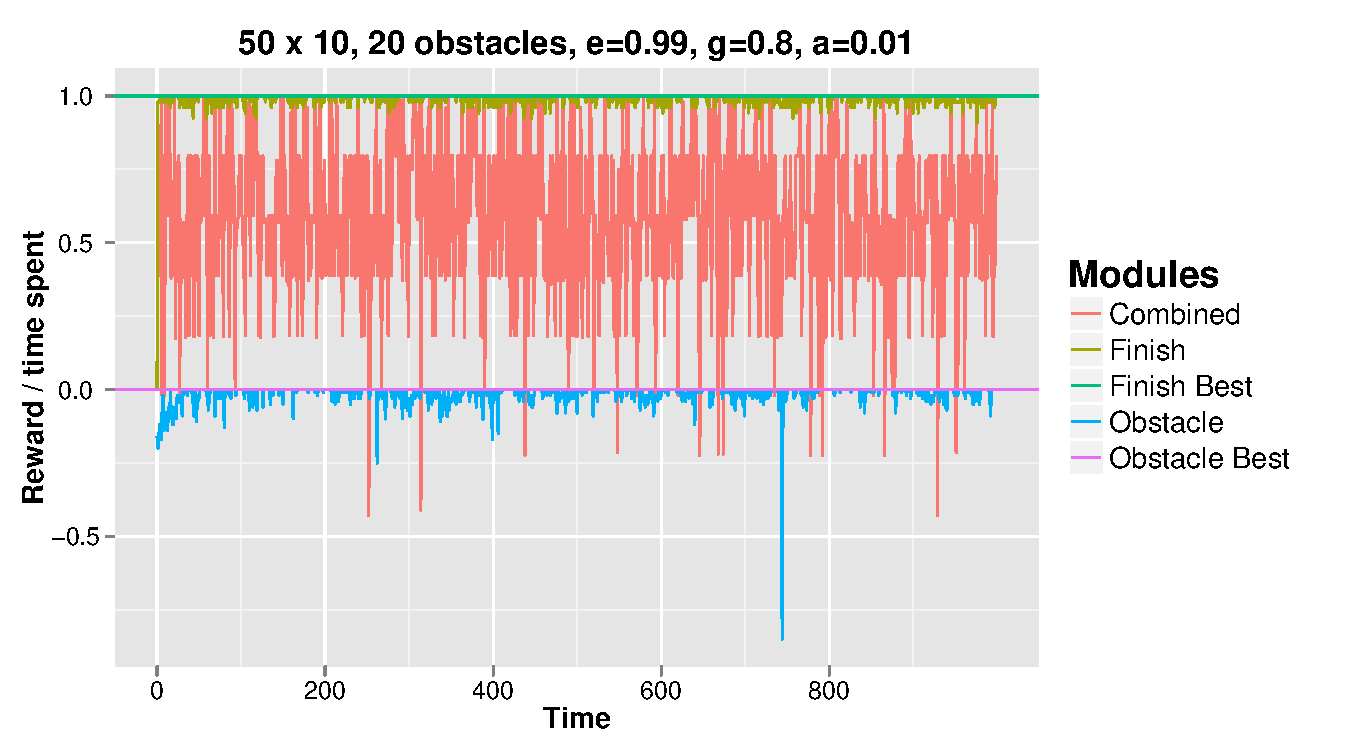
\includegraphics[width=0.95\textwidth]{results/qlearn-s50x10-o20-e99.pdf}
  \caption{epsilon = 0.99}
  \label{fig:ep099}
\end{figure}

\noindent In Figure \ref{fig:ep099}, for example, we get much better results giving the algorithm high confidence in what it should do at each step, instead of sometimes doing something randomly.


Figuring out appropriate weights for each module's Q was hard, and I may still not have gotten the best weights. This should be part of the learning algorith, I think. The individual episodes should train the Q's, and the merged episodes should train the weights. I did have time to implement this, unfortunately.

\begin{figure}[H]
  \centering
  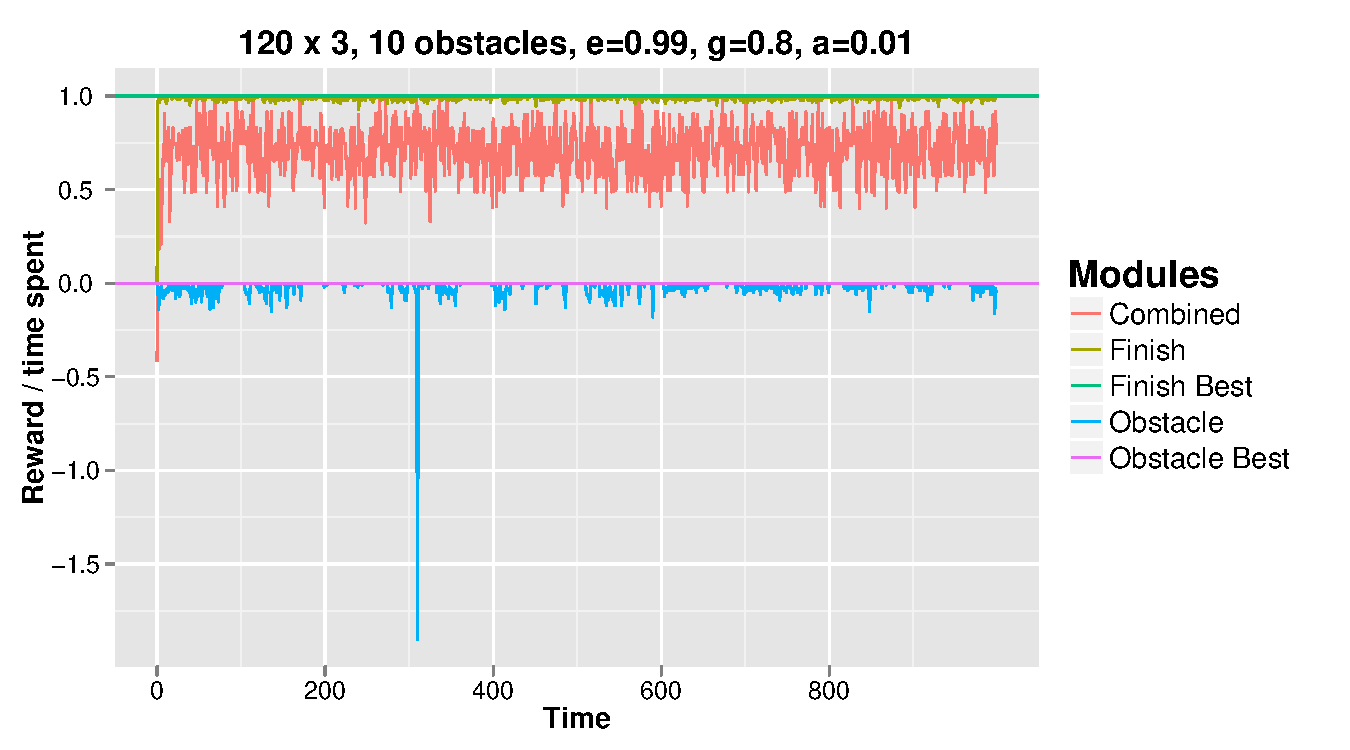
\includegraphics[width=0.95\textwidth]{results/qlearn-s120x3-o10.pdf}
  \caption{weight = 5/1 obstacle/figure}
\end{figure}

\begin{figure}[H]
  \centering
  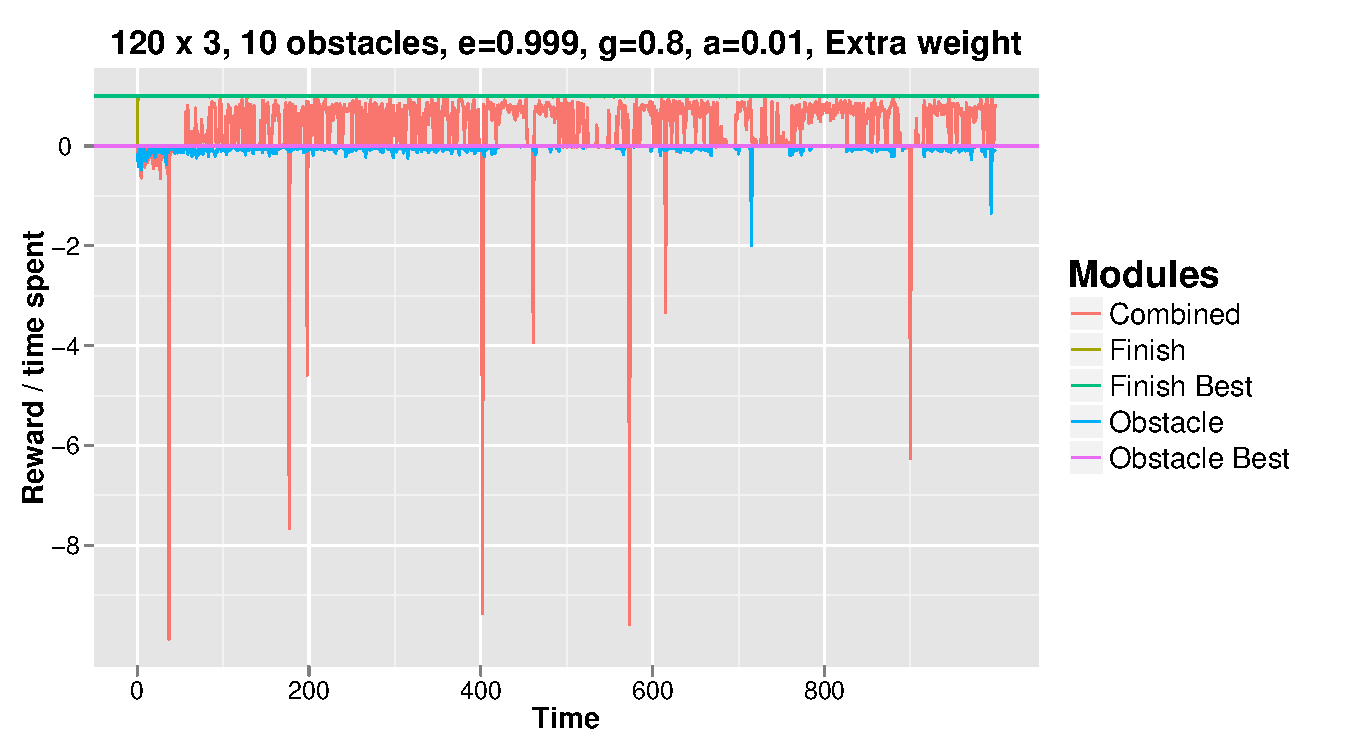
\includegraphics[width=0.95\textwidth]{results/qlearn-s120x3-o10-w50.pdf}
  \caption{weight = 50/1 obstacle/figure}
\end{figure}

I made the state space more nuanced for the following test; in this one, instead of looking at just the candidate to the right, the agent could looks at the three blocks one-away, and five blocks two-away, in each direction. Presumably, this would help with being able to keep the epsilon low, since the probability of doing something stupid (random) twice in a row is epsilon$^2$. It turns out that this does help quite a bit, though it takes longer to learn; see Figure \ref{fig:two-away}.

\begin{figure}[H]
  \centering
  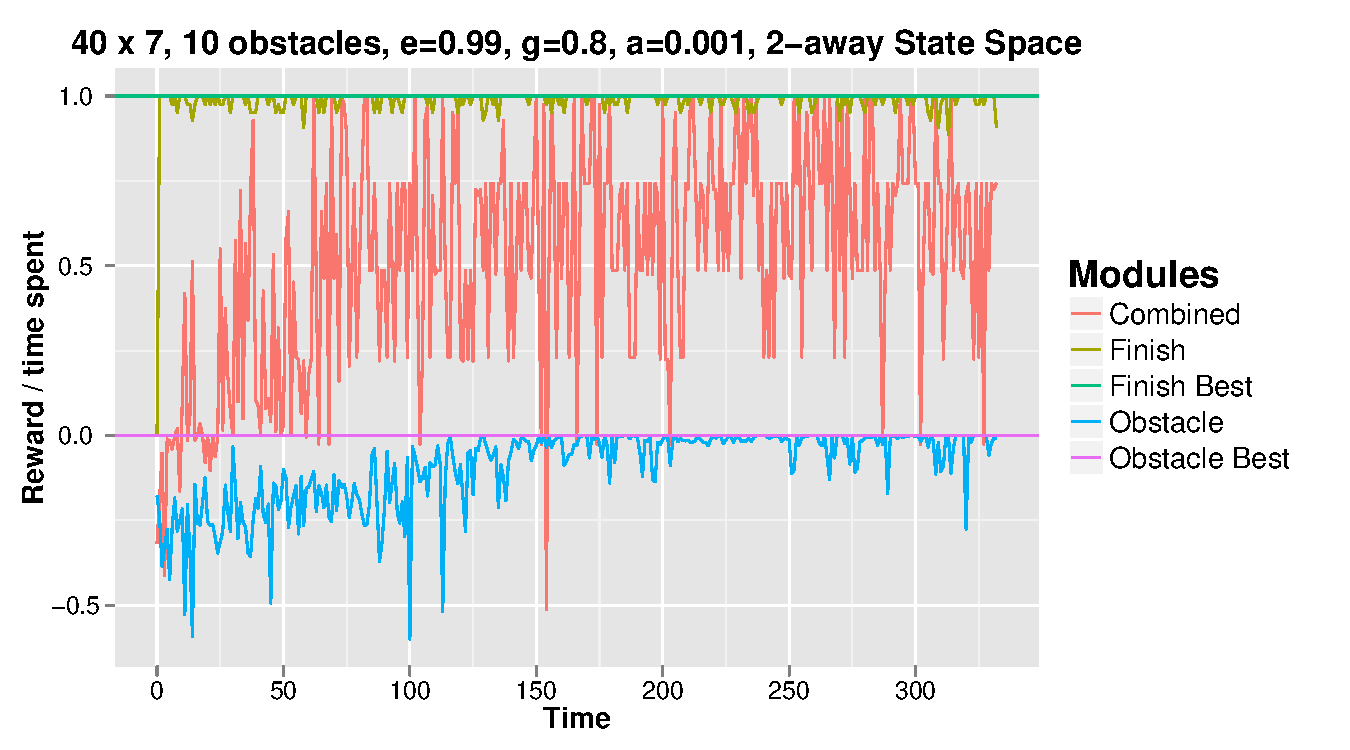
\includegraphics[width=0.95\textwidth]{results/qlearn-s40x7-o10-e99-directions.pdf}
  \caption{Two-away obstacle state space visibility}
  \label{fig:two-away}
\end{figure}

Certainly, it takes longer to train, but the result seems reassuring.

Here's another case, with much higher penalties; not a whole lot changes, and the reason why the Combined trend is so far underneath the Obstacle trend is because the Combined module doesn't account for time; if it was smart, if it accidentally hit more than one obstacle, it would hover around the end until the time was almost up, and then finish. But it's not smart (it doesn't know about the $reward / time$ metric), so it finishes as quickly as possible.

\begin{figure}[H]
  \centering
  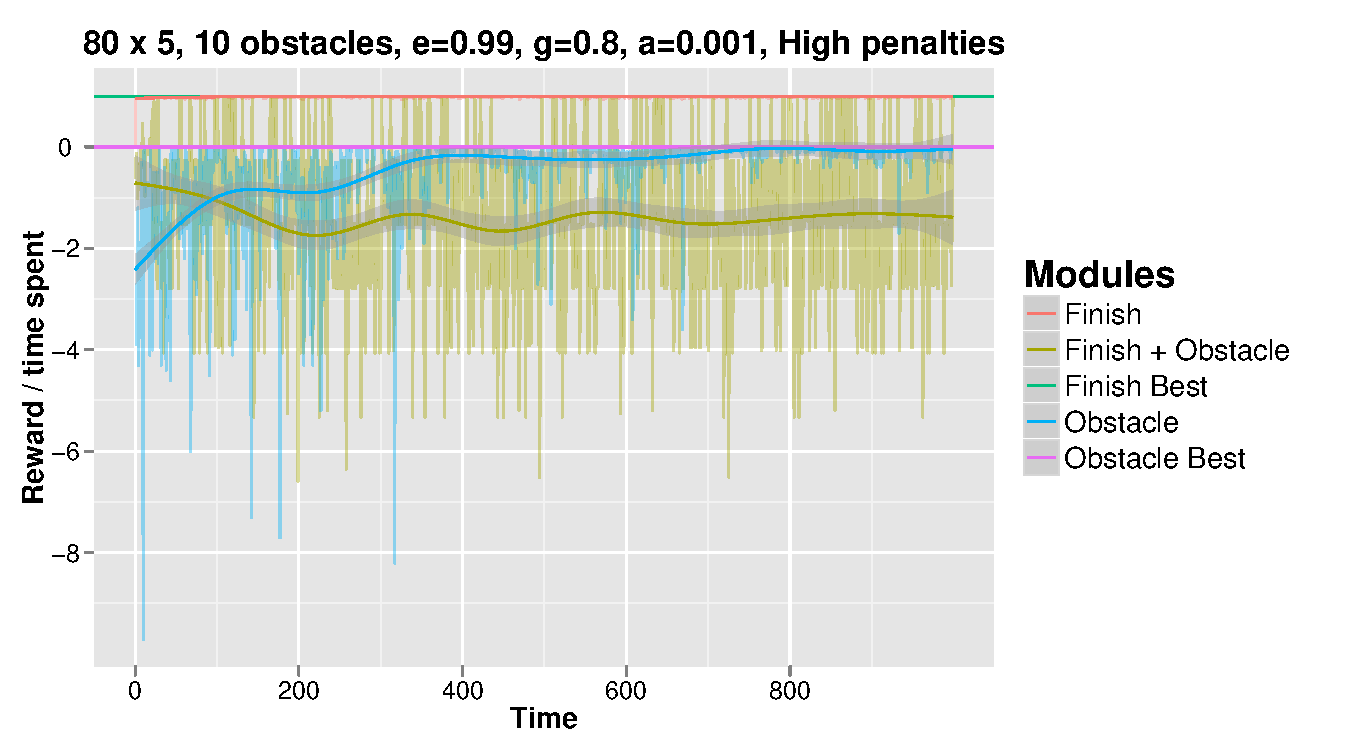
\includegraphics[width=0.95\textwidth]{results/qlearn-s80x5-o10-e0-99-a0-001-g0-8-high.pdf}
  \caption{High penalties of -100}
\end{figure}

If I set the penalty lower, the results suddenly \emph{look} a lot better:

\begin{figure}[H]
  \centering
  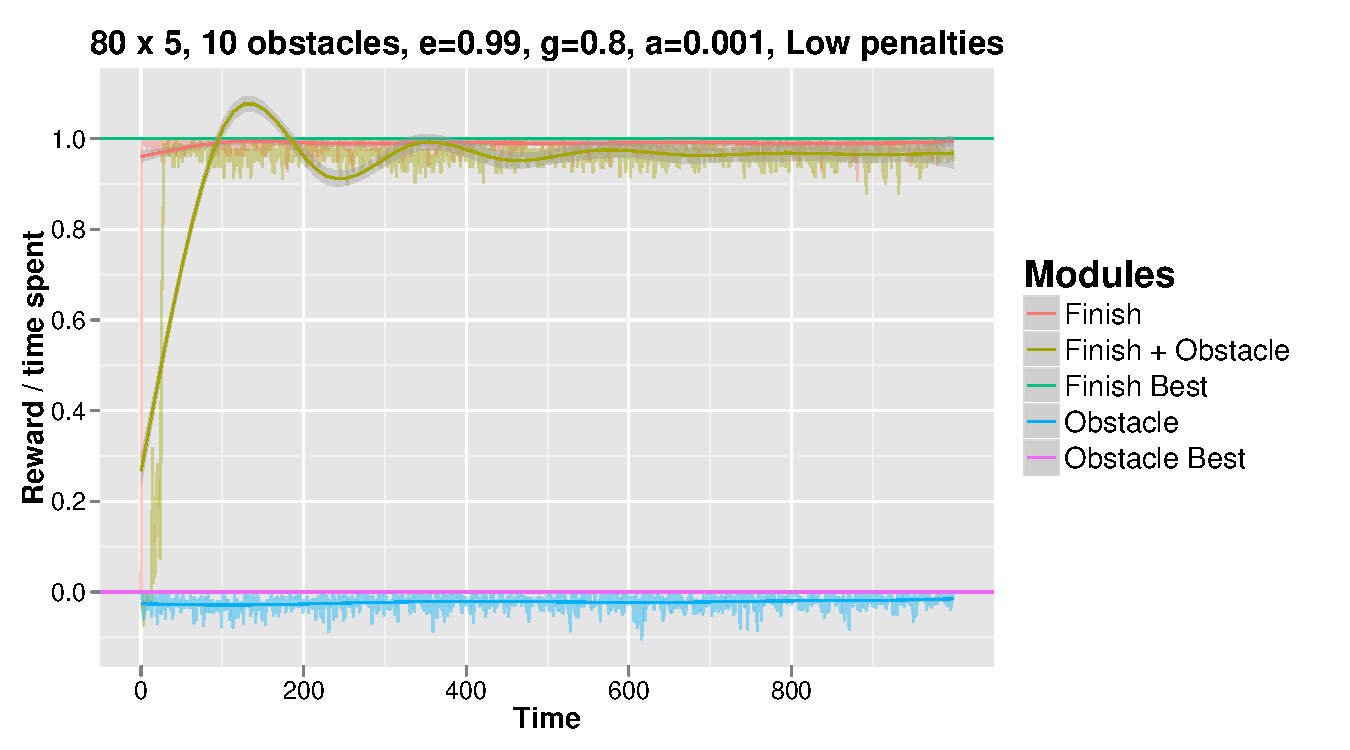
\includegraphics[width=0.95\textwidth]{results/qlearn-s80x5-o10-e0-99-a0-001-g0-8-low.pdf}
  \caption{Low penalties of -1}
\end{figure}



\section{Pitfalls}

There were a couple of hacks that I had to build into my algorithm:
\begin{enumerate}[a.]
  \item Often in the very first runs of the \texttt{finish} module, the agent would jitter left and right while running the width of the sidewalk several times, not making any forward progress. As far as I can tell, this was due to tiny differences between the score for going left as opposed to right, in the range of $< 0.0001$. Of course, sorting will register tiny differences just as significant as more reasonable (0.5) differences, so my hack was to pick a random action if the advantage between choosing the best and the second best actions was $< 0.001$.

  I could have accomplished the same thing by adding a very amount of noise, e.g. $\mathcal{N}(0, 0.001)$, to the Q function, but the threshold solution was easier and faster.

  \item Somewhat relatedly, when the \texttt{obstacle} module was running, the agent would sometimes hug the starting edge of the sidewalk. Because there was no penalty for running in that direction, and there could be a penalty for hitting an obstacle, that's a reasonable strategy. I tried handing out small penalties for running off the edges, but this didn't noticeably help performanace overall, and this bad habit was rare, so I didn't include these penalties in the analyses above.
\end{enumerate}

\section{Code}

I coded the homework in Python. Python is awesome because it lets you have multiple functions, each able to call the others, in \emph{one} file! This feature, unfortunately, is not shared by all languages used in this class.

The code is nothing clever. However, there is a fun curses-powered visualization; simply run the script with `draw' as one of the arguments: \texttt{python qlearn.py draw}. The program is much faster without this viz functionality, though. Also, you can easily configure the environment parameters via a filename: \texttt{python qlearn.py s20x5-o20-e0.9-a0.01-g0.8-out.csv} will create a 20-long by 5-wide sidewalk with 20 obstacles, an epsilon parameter of 0.9, etc. (same abbreviations as above).
In the output, I have created a trail for the agent, `a' and `.', which correspond to his previous two positions.

\begin{figure}[H]
  \centering
  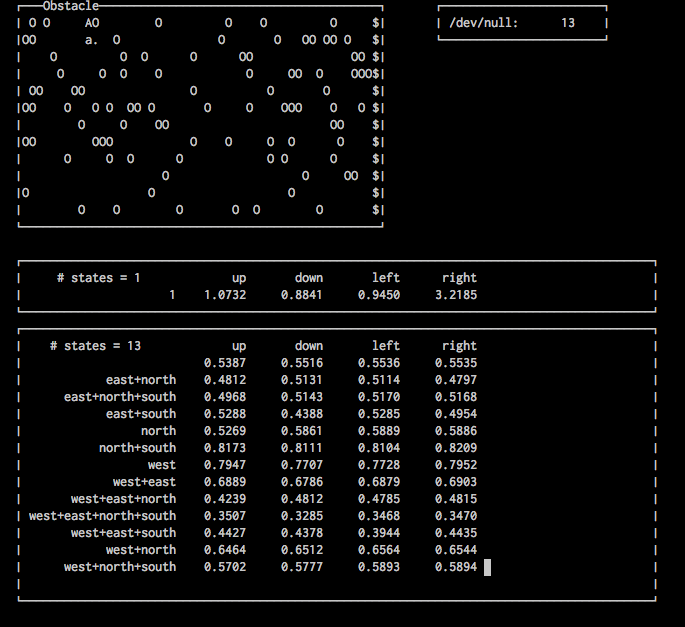
\includegraphics[width=0.95\textwidth]{curses.png}
  \caption{Screenshot of visualization.}
\end{figure}

\end{document}
